\section{\textit{K Nearest Neighbor}}
\subsection{Pengertian \textit{K Nearest Neighbor}}
\textit{K Nearest Neighbor} atau biasa disebut dengan KNN merupakan salah satu algoritma \textit{supervised learning}, dimana \textit{supervised learning} merupakan sebuah teknik pendekatan dengan sudah terdapat data latih, variabel yang ditargetkan dengan tujuan mengelompokkan suatu data ke data yang sudah ada. KNN biasanya digunakan untuk melakukan proses klasifikasi sebuah obyek/data baru dengan berdasarkan pada atribut dan sampel \textit{training}, dan berdasarkan kedekatan jarak antara data yang akan dievaluasi dengan k (tetangga/\textit{neighbor}) pada data latih (\textit{training})(\cite{hermaduanti2008sistem}).

\subsection{Kelebihan dan Kekurangan \textit{K Nearest Neighbor}}
\begin{enumerate}
    \item Kelebihan
\begin{itemize}
        \item Sangat sederhana implementasi.
        \item Kuat dalam hal ruang pencarian, misalnya, kelas tidak harus linear dipisahkan.
        \item Sangat Non Linear
        \par KNN merupakan salah satu algoritma yang bersifat non parametrik, yang artinya tidak mengasumsikan tentang distribusi dari \textit{isntance} pada \textit{dataset}. Model ini memiliki kelebihan pada model yang dihasilkan yaitu berdifat fleksibel dan non linear.
        \begin{figure}[!htpb]
        \centering
        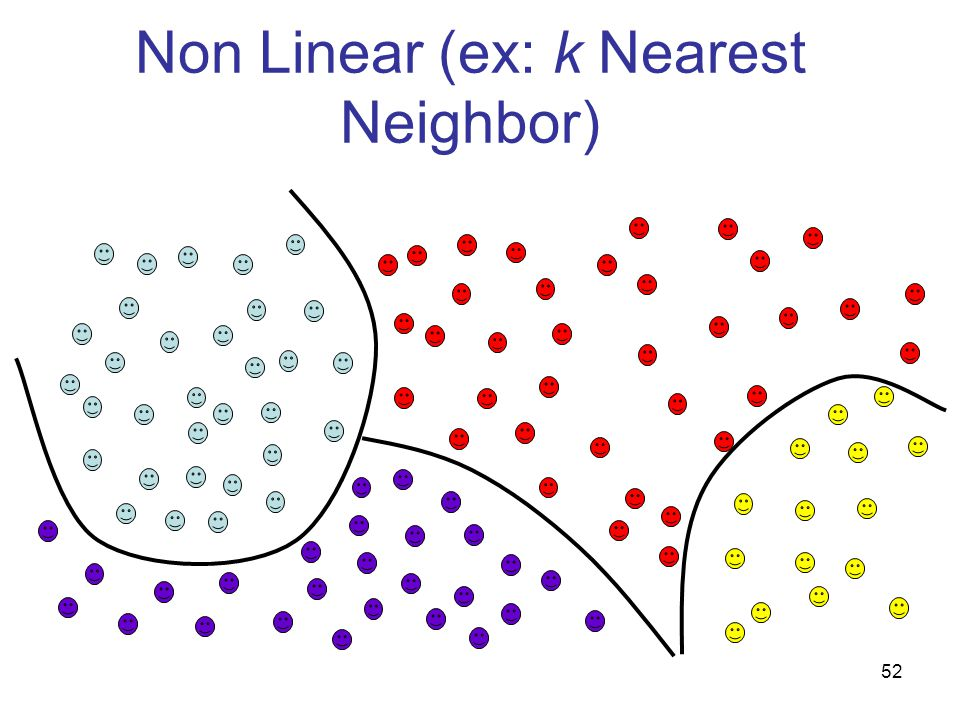
\includegraphics[width=6cm, height=4cm]{figures/knn.jpg}
        \caption{Non Linear
        \label{eq:31}}
        \end{figure} 
        \item Efektif untuk menghitung data dalam skala kecil.
        \item Beberapa parameter untuk acuan : jarak metrik dan k \cite{lestari2015penerapan}.
\end{itemize}
\item Kekurangan
    \begin{itemize}
        \item Perlu untuk menentukan nilai k yang optimal sehingga untuk menyatakan jumlah
tatangga terdekatnya lebih mudah.
        \item  Biaya komputasi yang cukup tinggi karena perhitungan jarak harus dilakukan pada setiap \textit{querry instance}\cite{afandie2014implementasi}.
    \end{itemize}
\end{enumerate}
\subsection{Langkah-langkah dalam Klasifikasi \textit{K Nearest Neighbor}}
\begin{enumerate}
    \item Tentukan parameter K (jumlah tetangga paling dekat).
    \item Hitung kuadrat jarak euclid masing – masing objek terhadap data sample yang
diberikan. Rumus yang digunakan adalah sebagai berikut:
    \begin{equation}
        D(a,b)= \sqrt{\sum_{k=1}^{d}(a_{k}-b_{k})^{2}}
        \label{rumusknn1}
    \end{equation}
    \par Dimana D(a,b) merupakan jarak skalar dari dua buah vektor antara data a dan data b yang berbentuk matrik dengan ukuran d dimensi.
    \item Urutkan objek – objek kedalam kelompok yang memiliki jarak terkecil.
    \item Kumpulkan kategori Y (Klasifikasi nearest neighbor).
    \item Dengan kategori nearest neighbor yang paling banyak, maka dapat diprediksikan
nilai query instance yang telah dihitung\cite{zainuddin2019implementasi}.
\end{enumerate}
Berikut merupakan penerapan contoh perhitungan K-Nearest Neighbor pada contoh soal untuk menentukan kelas Baik atau Buruk. Pada tabel \ref{knn1} merupakan data \textit{training} yang akan digunakan.
\begin{table}[!ht]
\centering
\caption{Contoh Data \textit{Training} pada KNN}
\label{knn1}
\begin{tabular}{|l|l|l|}
\hline
A1 & A2 & Y     \\ \hline
7  & 7  & BURUK \\ \hline
7  & 4  & BURUK \\ \hline
3  & 4  & BAIK  \\ \hline
1  & 4  & BAIK  \\ \hline
\end{tabular}
\end{table}
Diketahui sebuah data yang akan dicari hasil klasifikasinya, perhatikan pada tabel \ref{knn2}.
\begin{table}[!ht]
\centering
\caption{Contoh Data \textit{Testing} KNN}
\label{knn2}
\begin{tabular}{|l|l|l|}
\hline
A1 & A2 & Y   \\ \hline
3  & 7  & ..? \\ \hline
\end{tabular}
\end{table}
Ikuti langkah-langkah yang sebelumnya sudah dijelaskan, yakni sebagai berikut:
\begin{enumerate}
    \item Tentukan parameter k (jumlah tetangga terdekat), misal k=3
    \item Hitung jarak antara data baru dengan semua data \textit{training} mengggunakan rumus \ref{rumusknn1}, Perhatikan tabel \ref{knn3}.
    \begin{table}[!ht]
    \centering
    \caption{Jarak Eucliden}
    \label{knn3}
\begin{tabular}{|l|l|l|}
\hline
A1 & A2 & Eucliden(3,7)               \\ \hline
7  & 7  & (7-3)$^{2}$ + (7-7)$^{2}$= 16 \\ \hline
7  & 4  & (7-3)$^{2}$ + (4-7)$^{2}$= 25 \\ \hline
3  & 4  & (3-3)$^{2}$ + (4-7)$^{2}$= 9 \\ \hline
1  & 4  & (1-3)$^{2}$ + (4-7)$^{2}$= 13 \\ \hline
\end{tabular}
\end{table}
\item Setelah diperoleh nilai \textit{Eucliden}, kemudian urutkan nilai jarak tersebut dan tetapkan tetangga yang terdekat berdasarkan dengan jarak minimum ke k
\begin{table}[!ht]
    \centering
    \caption{Rank Jarak}
    \label{knn3}
\begin{tabular}{|l|l|l|l|l|}
\hline
A1 & A2 & Eucliden(3,7)               & Rank & 3 tetangga terdekat? \\ \hline
7  & 7  & (7-3)$^{2}$ + (7-7)$^{2}$= 16 & 3    & Ya                   \\ \hline
7  & 4  & (7-3)$^{2}$ + (4-7)$^{2}$= 25 & 4    & Tidak                \\ \hline
3  & 4  & (3-3)$^{2}$ + (4-7)$^{2}$= 9  & 1    & Ya                   \\ \hline
1  & 4  & (1-3)$^{2}$ + (4-7)$^{2}$= 13 & 2    & Ya                   \\ \hline
\end{tabular}
\end{table}
\pagebreak
\item Kemudian perhatikan kelas dari tetangga tersebut, nilai klasifikasi yang paling banyak pada tetangga terdekat merupakan hasil klasifikasi dari data \textit{testing}
\begin{table}[!ht]
    \centering
    \caption{Hasil Klasifikasi}
    \label{knn3}
\begin{tabular}{|l|l|l|l|l|l|}
\hline
A1 & A2 & Eucliden(3,7)               & Rank & 3 tetangga terdekat? & Y             \\ \hline
7  & 7  & (7-3)$^{2}$ + (7-7)$^{2}$= 16 & 3    & Ya                   & Buruk         \\ \hline
7  & 4  & (7-3)$^{2}$ + (4-7)$^{2}$= 25 & 4    & Tidak                & -             \\ \hline
3  & 4  & (3-3)$^{2}$ + (4-7)$^{2}$= 9  & 1    & Ya                   & \textbf{Baik} \\ \hline
1  & 4  & (1-3)$^{2}$ + (4-7)$^{2}$= 13 & 2    & Ya                   & \textbf{Baik} \\ \hline
\end{tabular}
\end{table}
\end{enumerate}
Maka dapat disimpulkan bahwa data dengan nilai A1=3 dan A2=7 memiliki hasil klasifikasi \textbf{baik}.

\subsection{Soal Latihan}
\begin{enumerate}
    \item Sebuah rumah tepat berada di antara kota dan kabupaten, pemerintah bingung menentukan posisi rumah apakah termasuk ke dalam daerah kota atau kabupatan. Tentukan posisi rumah berada di daerah mana?
    \begin{table}[!htpb]
    \centering
\begin{tabular}{|l|l|l|l|}
\hline
Rumah & Langitude & Longitude & Lokasi    \\ \hline
A     & 11        & 26        & Kota      \\ \hline
B     & 15        & 29        & Kota      \\ \hline
C     & 19        & 28        & Kota      \\ \hline
D     & 18        & 30        & Kota      \\ \hline
E     & 16        & 26        & Kota      \\ \hline
F     & 23        & 25        & Kabupaten \\ \hline
G     & 25        & 22        & Kabupaten \\ \hline
H     & 21        & 24        & Kabupaten \\ \hline
I     & 29        & 24        & Kabupaten \\ \hline
Z     & 19        & 25        & .....?    \\ \hline
\end{tabular}
\end{table}
\end{enumerate}
\pagebreak
\section{\textit{Naive Bayes Classifier}}
\subsection{Pengertian \textit{Naive Bayes Classifier}}
\textit{Naive Bayes Classifier} merupakan salah satu metode klasifikasi probabilistik dan statistik yang dikemukakan oleh Thomas Bayes. Algoritma \textit{Naive Bayes} biasa digunakan untuk memprediksi peluang di masa depan  berdasarkan pengalaman di masa sebelumnya (Teorema \textit{Bayes}) dengan asumsi independensi (ketidaktergantungan) yang kuat (naif)\cite{saleh2015implementasi}.
\subsection{Kelebihan dan Kekurangan \textit{Naive Bayes}}
\begin{enumerate}
    \item Kelebihan
    \begin{itemize}
        \item Dapat menangani data kuantitatif dan data diskrit.
        \item Dapat menggunakan sedikit data \textit{training} untuk pengestimasian parameter yang dibutuhkan untuk klasifikasi.
        \item Lebih Cepat dan Efisien \cite{hidayat2018klasifikasi}.
    \end{itemize}
    \item Kekurangan
    \begin{itemize}
        \item Tidak berlaku apabila memiliki nilai probabilitas 0 (nol), sehingga prediksi juga bernilai nol.
        \item Asumsi variabel yang bebas\cite{akbar2017prediksi}.
    \end{itemize}
\end{enumerate}
Persamaan dari teorema \textit{Bayes} adalah:
\begin{equation}
P(H|X) = \frac{P(X|H)P(H)}{P(X)} \\
\end{equation}
Keterangan : 
\par X 		: Data dengan class yang belum diketahui 
\par H 		: Hipotesis data merupakan suatu class spesifik 
\par P(H|X) 	: Probabilitas hipotesis H berdasar kondisi X (posteriori       probabilitas) 
\par P(H) 		: Probabilitas hipotesis H (prior probabilitas) 
\par P(X|H) 	: Probabilitas X berdasarkan kondisi pada hipotesis H 
\par P(X) 	: Probabilitas X 
\par Persamaan \textit{Naive Bayes} adalah:
\begin{equation}
    P(X|C_{i})=\prod_{k=1}^{n}P(x_{k}|C_{i})
    \label{rumus2}
\end{equation}
\subsection{Langkah-langkah dalam Klasifikasi \textit{Naive Bayes}}
Dalam melakukan klasifikasi \textit{Naive Bayes} berikut tahapan-tahapan yang harus dilakukan \cite{kosasih2018pengklasifikasian}:
Berikut adalah contoh data yang akan digunakan, perhatikan pada tabel \ref{contohdata}.
\begin{table}[!ht]
\centering
\caption{Contoh Data \textit{Training}}
\label{contohdata}
\begin{tabular}{|l|l|l|l|l|}
\hline
Umur             & Pendapatan & Mhs   & Rating Kredit & Beli Komputer \\ \hline
\textless{}=30   & tinggi     & bukan & fair          & tdk           \\ \hline
\textless{}=30   & tinggi     & bukan & excellent     & tdk           \\ \hline
30…40            & tinggi     & bukan & fair          & ya            \\ \hline
\textgreater{}40 & sedang     & bukan & fair          & ya            \\ \hline
\textgreater{}40 & rendah     & ya    & fair          & ya            \\ \hline
\textgreater{}40 & rendah     & ya    & excellent     & tdk           \\ \hline
31…40            & rendah     & ya    & excellent     & ya            \\ \hline
\textless{}=30   & sedang     & bukan & fair          & tdk           \\ \hline
\textless{}=30   & rendah     & ya    & fair          & ya            \\ \hline
\textgreater{}40 & sedang     & ya    & fair          & ya            \\ \hline
\textless{}=30   & sedang     & ya    & excellent     & ya            \\ \hline
31…40            & sedang     & bukan & excellent     & ya            \\ \hline
31…40            & tinggi     & ya    & fair          & ya            \\ \hline
\textgreater{}40 & sedang     & bukan & excellent     & tdk           \\ \hline
\end{tabular}
\end{table}
Misalkan ada sebuah data \textit{testing} yang ingin diketahui masuk ke dalam hasil klasifikasi mana, berikut contoh data \textit{testing} yang akan digunakan, perhatikan pada tabel \ref{testing}
\begin{table}[!ht]
\centering
\caption{Contoh Data \textit{Testing}}
\label{testing}
\begin{tabular}{|l|l|l|l|l|}
\hline
Umur           & Pendapatan & Mhs & Rating Kredit & Beli Komputer \\ \hline
\textless{}=30 & sedang     & ya  & fair          & ...?          \\ \hline
\end{tabular}
\end{table}
\par Langkah selanjutnya, dengan menghitung nilai $P(X_{k}|C_{i})$ pada setiap \textit{class}.

\begin{enumerate}
    \item $P(umur :\textless{}=30|Beli Komputer)$
    \par Perhatikan pada tabel \ref{prob1} pada kolom Umur, diperoleh bahwa probabilitas Umur dengan $\textless{}=30$ terhadap kelas beli komputer dengan nilai ya adalah sebanyak 2 data, dan untuk kelas beli komputer dengan nilai tidak sebanyak 3 data. Nilai probabilitasnya yakni sebagai berikut:
\par $P(umur :\textless{}=30|Beli Komputer:Ya)$ = 2/9 = 0.220
\par $P(umur :\textless{}=30|Beli Komputer:Tidak)$ = 3/5 = 0.600
\par nilai 9 merupakan jumlah data dengan kelas Ya sebanyak 9, dan nilai 5 merupakan jumlah data dengan kelas Tidak sebanyak 5.
\item $P(pendapatan :sedang|Beli Komputer)$
\par Perhatikan pada tabel \ref{prob2} pada kolom Pendapatan, diperoleh bahwa probabilitas Umur dengan $\textless{}=30$ terhadap kelas beli komputer dengan nilai ya adalah sebanyak 4 data, dan untuk kelas beli komputer dengan nilai tidak sebanyak 2 data. Nilai probabilitasnya yakni sebagai berikut:
\par $P(pendapatan :sedang|Beli Komputer:Ya)$ = 4/9= 0.444
\par $P(pendapatan :sedang|Beli Komputer:Tidak)$ = 2/5=0.400

\item $P(Mhs:ya|Beli Komputer)$
\par Perhatikan pada tabel \ref{prob2} pada kolom Mhs, diperoleh bahwa probabilitas Umur dengan $\textless{}=30$ terhadap kelas beli komputer dengan nilai ya adalah sebanyak 6 data, dan untuk kelas beli komputer dengan nilai tidak sebanyak 1 data. Nilai probabilitasnya yakni sebagai berikut:
\par $P(Mhs:ya|Beli Komputer:Ya)$ = 6/9 =  0.670 
\par $P(Mhs:ya|Beli Komputer:Tidak)$ = 1/5	 =  0.200

\item $P(Ratingkredit:Fair|Beli Komputer)$
\par Perhatikan pada tabel \ref{prob2} pada kolom Rating Kredit, diperoleh bahwa probabilitas Umur dengan $\textless{}=30$ terhadap kelas beli komputer dengan nilai ya adalah sebanyak 6 data, dan untuk kelas beli komputer dengan nilai tidak sebanyak 2 data. Nilai probabilitasnya yakni sebagai berikut:
\par $P(Ratingkredit:Fair|Beli Komputer:Ya)$ = 6/9	=  0.670
\par $P(Ratingkredit:Fair|Beli Komputer:Tidak)$ = 2/5  =  0.400
    \begin{table}[!ht]
    \centering
    \caption{Hitung Nilai Probabilitas $P(umur :\textless{}=30|Beli Komputer)$ }
    \label{prob1}
\begin{tabular}{|l|l|l|l|l|}
\hline
\textbf{Umur}             & Pendapatan & Mhs   & Rating Kredit & Beli Komputer \\ \hline
\textbf{\textless{}=30}   & tinggi     & bukan & fair          & tdk           \\ \hline
\textbf{\textless{}=30}   & tinggi     & bukan & excellent     & tdk           \\ \hline
\textbf{\textless{}=30}   & sedang     & bukan & fair          & tdk           \\ \hline
\textbf{\textless{}=30}   & rendah     & ya    & fair          & ya            \\ \hline
\textbf{\textless{}=30}   & sedang     & ya    & excellent     & ya            \\ \hline
\textbf{\textgreater{}40} & rendah     & ya    & excellent     & tdk           \\ \hline
\textbf{\textgreater{}40} & sedang     & bukan & fair          & ya            \\ \hline
\textbf{\textgreater{}40} & rendah     & ya    & fair          & ya            \\ \hline
\textbf{\textgreater{}40} & sedang     & ya    & fair          & ya            \\ \hline
\textbf{\textgreater{}40} & sedang     & bukan & excellent     & tdk           \\ \hline
\textbf{30…40}            & tinggi     & bukan & fair          & ya            \\ \hline
\textbf{31…40}            & rendah     & ya    & excellent     & ya            \\ \hline
\textbf{31…40}            & sedang     & bukan & excellent     & ya            \\ \hline
\textbf{31…40}            & tinggi     & ya    & fair          & ya            \\ \hline
\end{tabular}
\end{table}



\begin{table}[!ht]
\centering
\caption{Hitung Nilai Probabilitas $P(pendapatan :sedang|Beli Komputer)$ }
\label{prob2}
\begin{tabular}{|l|l|l|l|l|}
\hline
Umur             & \textbf{Pendapatan} & Mhs   & Rating Kredit & Beli Komputer \\ \hline
\textgreater{}40 & \textbf{rendah}     & ya    & excellent     & tdk           \\ \hline
\textless{}=30   & \textbf{rendah}     & ya    & fair          & ya            \\ \hline
\textgreater{}40 & \textbf{rendah}     & ya    & fair          & ya            \\ \hline
31…40            & \textbf{rendah}     & ya    & excellent     & ya            \\ \hline
\textless{}=30   & \textbf{sedang}     & bukan & fair          & tdk           \\ \hline
\textgreater{}40 & \textbf{sedang}     & bukan & excellent     & tdk           \\ \hline
\textless{}=30   & \textbf{sedang}     & ya    & excellent     & ya            \\ \hline
\textgreater{}40 & \textbf{sedang}     & bukan & fair          & ya            \\ \hline
\textgreater{}40 & \textbf{sedang}     & ya    & fair          & ya            \\ \hline
31…40            & \textbf{sedang}     & bukan & excellent     & ya            \\ \hline
\textless{}=30   & \textbf{tinggi}     & bukan & fair          & tdk           \\ \hline
\textless{}=30   & \textbf{tinggi}     & bukan & excellent     & tdk           \\ \hline
30…40            & \textbf{tinggi}     & bukan & fair          & ya            \\ \hline
31…40            & \textbf{tinggi}     & ya    & fair          & ya            \\ \hline
\end{tabular}
\end{table}


\begin{table}[!ht]
\centering
\caption{Hitung Nilai Probabilitas $P(Mhs:ya|Beli Komputer)$ }
\label{prob2}
\begin{tabular}{|l|l|l|l|l|}
\hline
Umur             & Pendapatan & \textbf{Mhs}   & Rating Kredit & Beli Komputer \\ \hline
\textless{}=30   & sedang     & \textbf{bukan} & fair          & tdk           \\ \hline
\textgreater{}40 & sedang     & \textbf{bukan} & excellent     & tdk           \\ \hline
\textless{}=30   & tinggi     & \textbf{bukan} & fair          & tdk           \\ \hline
\textless{}=30   & tinggi     & \textbf{bukan} & excellent     & tdk           \\ \hline
\textgreater{}40 & sedang     & \textbf{bukan} & fair          & ya            \\ \hline
31…40            & sedang     & \textbf{bukan} & excellent     & ya            \\ \hline
30…40            & tinggi     & \textbf{bukan} & fair          & ya            \\ \hline
\textgreater{}40 & rendah     & \textbf{ya}    & excellent     & tdk           \\ \hline
\textless{}=30   & rendah     & \textbf{ya}    & fair          & ya            \\ \hline
\textgreater{}40 & rendah     & \textbf{ya}    & fair          & ya            \\ \hline
31…40            & rendah     & \textbf{ya}    & excellent     & ya            \\ \hline
\textless{}=30   & sedang     & \textbf{ya}    & excellent     & ya            \\ \hline
\textgreater{}40 & sedang     & \textbf{ya}    & fair          & ya            \\ \hline
31…40            & tinggi     & \textbf{ya}    & fair          & ya            \\ \hline
\end{tabular}
\end{table}



\begin{table}[!ht]
\centering
\caption{Hitung Nilai Probabilitas $P(Ratingkredit:Fair|Beli Komputer)$}
\label{prob2}
\begin{tabular}{|l|l|l|l|l|}
\hline
Umur             & Pendapatan & Mhs   & \textbf{Rating Kredit} & Beli Komputer \\ \hline
\textless{}=30   & tinggi     & bukan & \textbf{excellent}     & tdk           \\ \hline
\textgreater{}40 & sedang     & bukan & \textbf{excellent}     & tdk           \\ \hline
\textgreater{}40 & rendah     & ya    & \textbf{excellent}     & tdk           \\ \hline
31…40            & sedang     & bukan & \textbf{excellent}     & ya            \\ \hline
31…40            & rendah     & ya    & \textbf{excellent}     & ya            \\ \hline
\textless{}=30   & sedang     & ya    & \textbf{excellent}     & ya            \\ \hline
\textless{}=30   & sedang     & bukan & \textbf{fair}          & tdk           \\ \hline
\textless{}=30   & tinggi     & bukan & \textbf{fair}          & tdk           \\ \hline
\textgreater{}40 & sedang     & bukan & \textbf{fair}          & ya            \\ \hline
30…40            & tinggi     & bukan & \textbf{fair}          & ya            \\ \hline
\textless{}=30   & rendah     & ya    & \textbf{fair}          & ya            \\ \hline
\textgreater{}40 & rendah     & ya    & \textbf{fair}          & ya            \\ \hline
\textgreater{}40 & sedang     & ya    & \textbf{fair}          & ya            \\ \hline
31…40            & tinggi     & ya    & \textbf{fair}          & ya            \\ \hline
\end{tabular}
\end{table}
\pagebreak
\pagebreak
\par Setelah dihitung nilai  $P(X_{k}|C_{i})$, maka tahap selanjutnya menghitung nilai probabilitas kelas yang diperoleh setelah melakukan perhitungan probabilitas atribut terhadap kelas, berikut hasil perhitungannya pada table \ref{hasil1}
\begin{table}[!ht]
\centering
\caption{Hitung nilai probabilitas}
\label{hasil1}
\begin{tabular}{|l|l|}
\hline
\multicolumn{2}{|c|}{\begin{tabular}[c]{@{}c@{}}Hitung P(Xk | Ci)\\   utk setiap class I\end{tabular}} \\ \hline
P(umur\textless{}=30|beli\_komputer=ya)           = 2/9                    & 0.222                    \\ \hline
P(umur\textless{}=30|beli\_komputer=tdk)         = 3/5                      & 0.6                      \\ \hline
P(pendapatan=sedang|beli\_komputer=ya)      = 4/9                           & 0.444                    \\ \hline
P(pendapatan=sedang|beli\_komputer=tdk)     = 2/5                           & 0.4                      \\ \hline
P(mhs=ya|beli\_komputer=ya)      = 6/9                                      & 0.667                    \\ \hline
P(mhs=ya| beli\_komputer=tdk)     = 1/5                                     & 0.2                      \\ \hline
P(ratingkredit=fair| beli\_komputer=ya)      =6/9                           & 0.667                    \\ \hline
P(rating kredit=ya|beli\_komputer=tdk)     = 2/5                            & 0.4                      \\ \hline
\end{tabular}
\end{table}

\par Setelah diperoleh nilai probabilitas kelas, kemudian kalikan nilai probabilitas yang diperoleh terhadap nilai probabilitas kelas, berikut peehitungannya:
\par P(X|belicomputer=“ya”) * P(belicomputer=“ya”) = 0.044*(9/14) = 0.028
\par P(X|belicomputer=“tidak”) * P(belicomputer=“tidak”) = 0.044*(5/14)= 0.007

\par Setelah mengalikan nilai probabilitas,maka diperoleh hasil bahwa data sesuai pada tabel \ref{tab2} diklasifikasikan pada \textbf{Ya}, karena nilai probabilitas lebih besar dari pengujian yang lain.   

\end{enumerate}
\subsection{Soal Latihan}
\begin{enumerate}
    \item Kerjakan soal dibawah ini, tentukan \textit{class label} dari data dibawah ini, 
    \begin{table}[!ht]
    \centering
\begin{tabular}{|l|l|l|l|l|l|l|l|l|}
\hline
No & Nama                & A1 & A2 & A3 & A4 & A5 & A6 & Hasil \\ \hline
1  & Yoka Alit Kameswara & 2  & 4  & 3  & 2  & 3  & 6  & ....? \\ \hline
\end{tabular}
\end{table}
berikut penjelasan tentang atribut yang digunakan pada soal ini, perhatikan tabel \ref{soal1}
    \begin{table}[!ht]
    \centering
    \caption{Penjelasan Atribut Soal}
    \label{soal1}
\begin{tabular}{|l|l|l|l|l|}
\hline
No & Atribute                      & Nilai            & Label & Keterangan  \\ \hline
1  & Usia (A1)                     & Sangat Produktif & 3     & 15-49 tahun \\ \hline
   &                               & Produktif        & 2     & 50-64 tahun \\ \hline
   &                               & Tidak produktif  & 1     & 65 tahun    \\ \hline
2  & Pendidikan (A2)               & PT               & 4     &             \\ \hline
   &                               & SMA              & 3     &             \\ \hline
   &                               & SMP              & 2     &             \\ \hline
   &                               & SD               & 1     &             \\ \hline
3  & Pekerjaan (A3)                & Tetap            & 3     &             \\ \hline
   &                               & Tidak tetap      & 2     &             \\ \hline
   &                               & Tidak bekerja    & 1     &             \\ \hline
4  & Tanggungan (A4)               & \textless{}4     & 2     &             \\ \hline
   &                               & \textgreater{}4  & 1     &             \\ \hline
5  & Status kepemilikan Rumah (A5) & Milik sendiri    & 3     &             \\ \hline
   &                               & Sewa/Kontrak     & 2     &             \\ \hline
   &                               & Menumpang        & 1     &             \\ \hline
6  & Luas Rumah (A6)               & Tipe 120         & 6     &             \\ \hline
   &                               & Tipe 60          & 5     &             \\ \hline
   &                               & Tipe 54          & 4     &             \\ \hline
   &                               & Tipe 45          & 3     &             \\ \hline
   &                               & Tipe 36          & 2     &             \\ \hline
   &                               & Tipe 21          & 1     &             \\ \hline
\end{tabular}
\end{table}
    \begin{table}[!ht]
    \centering
\begin{tabular}{|l|l|l|l|l|l|l|l|l|}
\hline
No & Nama             & A1 & A2 & A3 & A4 & A5 & A6 & Hasil         \\ \hline
1  & Usep Heliana     & 3  & 2  & 3  & 2  & 1  & 6  & Pra Sejahtera \\ \hline
2  & A Rahmat         & 2  & 1  & 2  & 2  & 1  & 6  & Pra Sejahtera \\ \hline
3  & Ujang Tarman     & 3  & 1  & 3  & 2  & 3  & 6  & Sejahtera 1   \\ \hline
4  & Maimunah         & 3  & 3  & 1  & 2  & 1  & 6  & Pra Sejahtera \\ \hline
5  & Kasna            & 2  & 1  & 3  & 2  & 3  & 6  & Sejahtera 1   \\ \hline
6  & Wiwi             & 2  & 1  & 2  & 2  & 3  & 6  & Sejahtera 1   \\ \hline
7  & Mufti Handoko    & 3  & 4  & 3  & 2  & 3  & 6  & Sejahtera 2   \\ \hline
8  & Atam             & 1  & 3  & 3  & 2  & 3  & 6  & Sejahtera 1   \\ \hline
9  & Entis Sutisna    & 3  & 2  & 3  & 2  & 3  & 6  & Sejahtera 2   \\ \hline
10 & Jajang Supriatna & 3  & 3  & 3  & 2  & 3  & 6  & Sejahtera 2   \\ \hline
\end{tabular}
\end{table}
\end{enumerate}
\pagebreak
\par \textbf{Penyelesaian}
\begin{enumerate}
    \item Tentukan nilai probabilitas kelas terlebih dahulu, maka diperoleh nilai probabilitas sebagai berikut:
    \begin{table}[!ht]
    \centering
\begin{tabular}{|l|l|l|}
\hline
Kelas         & Jumlah Data & Probabilitas \\ \hline
Sejahtera 2   & 3           & 0.3          \\ \hline
Pra Sejahtera & 3           & 0.3          \\ \hline
Sejahtera 1   & 4           & 0.4          \\ \hline
Total         & 10          & 1            \\ \hline
\end{tabular}
\end{table}
\item Selanjutnya nilai probabilitas atribut terhadap kelas maka diperoleh sebagai berikut:
\begin{figure}[!htpb]
        \centering
        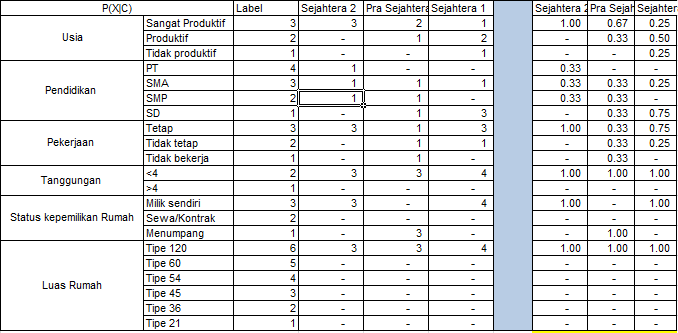
\includegraphics[width=10cm, height=5cm]{figures/probailitas.PNG}
        \end{figure} 
\item Tahap terakhir uji data yang akan dicari hasil klasifikasinya dengan mengalikan nilai probabilitas kelas dan probabilitas atribut terhadap kelas sesuai dengan nilai yang dimiliki oleh data.
% Please add the following required packages to your document preamble:
% \usepackage{multirow}
\begin{table}[!ht]
\centering
\begin{tabular}{|l|l|c|l|l|l|l|}
\hline
Nama                   & A1              & \multicolumn{1}{l|}{A2}   & A3  & A4  & A5  & A6  \\ \hline
Yoka Alit Kameswara Ir & 2               & \multicolumn{1}{l|}{4}    & 3   & 2   & 3   & 6   \\ \hline
\multicolumn{7}{|l|}{}                                                                       \\ \hline
Sejahtera 2            & 0.0023          & \multicolumn{5}{c|}{\multirow{}{}{Sejahtera 1}} \\ \cline{1-2}
Pra Sejahtera          & -               & \multicolumn{5}{c|}{}                             \\ \cline{1-2}
Sejahtera 1            & \textbf{0.0028} & \multicolumn{5}{c|}{}                             \\ \hline
\end{tabular}
\end{table}
\end{enumerate}
\section{Algoritma Apriori}
\subsection{Pengertian Algoritma Apriori}
Algoritma apriori merupakan jenis aturan asosiasi pada data mining, dimana aturan yang menyatakan asosiasi antara atribut-atribut yang disebut \textit{market basket analysis} \cite{ye2006parallel}. \textit{Asosiation rule} adalah teknik data minig yang digunakan untuk menentukan atura asosiatif antar suatu kombinasi \textit{item}. Algoritma apriori yang bertujuan untuk menemukan \textit{frequent itemsets} pada sekumpulan data yang memenuhi syarat minimum \textit{support} dan minimum \textit{confidence} yang telah ditentukan.
\par
Algoritma Apriori menggunakan pengetahuan frekuensi atribut yang  sebelumnya telah didapat untuk dilakukan proses informasi selanjutnya. Pada algoritma Apriori  menentukan kandidat yang mungkin muncul dengan cara memperhatikan nilai minimum \textit{support} dan nilai minimum \textit{confidence}. \textit{Support} adalah nilai pengunjung atau persentase kombinasi sebuah \textit{item} dalam \textit{database}. Sedangkan \textit{confidence} adalah nilai kepastian yang menentukan kuatnya hubungan antar \textit{item} dalam sebuah Apriori. \textit{Confidence} dapat dicari setelah pola frekuensi munculnya sebuah \textit{item} ditemukan.
\subsection{Kelebihan dan Kelemahan Algoritma Apriori}
\par Beberapa kelebihan yang dimiliki oleh algoritma apriori adalah sebagai berikut \cite{fauzy2016penerapan}:
 \begin{enumerate}
\item Menghasilkan kombinasi yang sangat banyak sehingga sangat tidak efisien. 
\item Lebih sederhana
\item Dapat menangani data yang besar
\item Apriori memiliki akurasi rules yang tinggi
\end{enumerate}

\par Beberapa kelemahan yang dimiliki oleh algoritma apriori adalah sebagai berikut:
 \begin{enumerate}
\item Proses \textit{scan database} yang dilakukan setiap kali iterasi, sehingga waktu yang diperlukan bertambah dengan makin banyak iterasi
\item Proses \textit{scanning} yang
dilakukan pada apriori yang berulang kali membuat tingkat kecepatan menjadi lambat

\end{enumerate}

\subsection{Tahap-Tahap Menghitung Algoritma Apriori}
Tahap-tahap yang dilakukan untuk mendapatkan \textit{frequent itemset} dalam algoritma apriori adalah sebagai berikut \cite{triyanto2014association}:
 \begin{enumerate}
\item Penggabungan (\textit{Join})
\par Proses penggabungan dilakukan dengan melakukan kombinasi terhadap satu \textit{item} dengan \textit{item} yang lainnya hingga tidak dapat terbentuk kombinasi lagi.
\item Pemangkasan (Prune)
\par proses pemangkasan merupakan hasil dari \textit{item} yang sudah dikombinasi kemudian dilakukan pemangkasan dengan menggunakan minimum \textit{support} yang telah ditentukan sebelumnya. 
\end{enumerate}

\par Prinsip-prinsip dalam algoritma apriori adalah sebagai berikut \cite{tampubolon2013implementasi}:
 \begin{enumerate}
\item Mengumpulkan \textit{item} tunggal kemudian mencari \textit{item} dengan nilai tersebar.
\item Mendapatkan \textit{candidate pairs} kemudian menghitung \textit{large pairs} dari setiap \textit{item} yang ada
\item Menemukan \textit{candidate triplets} dari setiap \textit{item} dan seterusnya
\item Setiap \textit{subset} dari sebuah \textit{frequent itemset} harus menjadi \textit{frequent}.
\end{enumerate}

\par Algoritma apriori terbagi menjadi beberapa tahap yaitu iterasi (\textit{pass}). Setiap iterasi mnghasilkan sebuah pola frekuensi tinggi dengan panjang yang sama dimulai dari iterasi pertama yang menghasilkan pola frekuensi tinggi dengan panjang satu. Pada iterasi pertama, nilai \textit{support} dari setiap \textit{item} didapat, \textit{item} yang memiliki nilai \textit{support} lebih besar dari nilai minimum \textit{support} akan diambil sebagai pola frekuensi tinggi dengan panjang satu atau 1-\textit{itemset}. 1-i artinya satu set yang terdiri dari k \textit{item}. Kemuidan untuk kandidat 2-\textit{itemset} akan dihitung nilai \textit{support}-nya dengan melakukan \textit{scan} terhadap \textit{database}.
\par
\textit{Support} yang diamksudkan disini artinya jumlah transaksi pada \textit{database} yang mengandung keduan \textit{item} dalam kandidat 2-\textit{itemset}. Setelah nilai \textit{support} dari semua kandidat 2-\textit{itemset} didapat, kandidat 2-\textit{itemset} yang memenuhi syarat nilai minimum \textit{support} dapat ditetapkan sebagai 2-\textit{itemset} yang merupakan pola frekuensi tinggi dengan panjang 2 \cite{nursikuwagus2016implementasi}.
\par
Untuk iterasi ke-k dapat dibagi menjadi beberapa bagian:
 \begin{enumerate}
\item Pembentukan kandidat \textit{itemset}.
\par Kandidat k-\textit{itemset} dibentuk dari kombinasi (k-1)-\textit{itemset} yang didapat dari iterasi sebelumnya. Karakteristik dari algoritma apriori adalah adanya pemangkaan terhadap kandidat k-iterasi yang subsetnya berisikan k-1 \textit{item} tidak termasuk kedalam pola frekuensi tinggi dengan panjang k-1.
\item Perhitungan nilai \textit{support} dari setiap kandidat k-\textit{itemset}.
\par Nilai \textit{support} dari setiap kandidat k-\textit{itemset} didapt dengan melakukan \textit{scan} terhadap \textit{database} untuk menghitung jumlah transaksi yang memuat seluruh \textit{item} didalam kandidat k-\textit{itemset} tersebut. Ini merupakan karakteristik dari algoritma ini dimana diperlukan perhitungn dengan melakukan \textit{scan} seluruh \textit{database} sebanyak k-\textit{itemset} terpanjang.
\item Menetapkan pola frekuensi tinggi.

\par 
Pola frekuensi tinggi yang memuat k \textit{item} atau k-\textit{itemset} ditetapkan dari kandidat k-\textit{itemset} yang nilai \textit{support}-nya lebih besar dari nilai minimum \textit{support} yang telah ditetapkan sebelumnya.
\item Apabila tidak mendapatkan pola frekuensi tinggi yang baru, maka semua proses berhenti. Bila tidak, makan k ditambah satu dan kembali ke bagian awal.
\end{enumerate}

\subsection{Rumus Algoritma Apriori}
\par Algoritma apriori menggunakan pengetahuan frekuensi atribut yang telah diketahui untuk selanjut dilakukan proses informai selanjutnya. Algoritma apriori melakukan penentuan kandidat yang mungkin muncul dengan cara memerhatikan nilai  minimum \textit{support} dan \textit{confidence} yang telah ditentukan sebelumnya \cite{yanto2015implementasi}.

\par 
\textbf{\textit{Support}}: sebuah ukuran yang menunjukkan besarnya tingkat dominasi sebuah \textit{item} atau \textit{itemset} dari keseluruhan transaksi. Ukuran ini akan menentukan kelayakan sebuah \textit{itemset} atau \textit{item} untuk dihitung nilai \textit{confidence} tersebut dapat digunakan untuk menentukan tingkat dminasi \textit{item} tunggal. Misalnya, semua tranaksi yang tersedia, berapa besar tingkat dominasi yang menunjukkan bahwa \textit{item} A \& B dibeli secara bersamaan.
\par
\textbf{\textit{Confidence}}: sebuahukuran yang menunjukkan hubungan antara kedua \textit{itemset} secara \textit{conditional}. Misalnya, seberapa sering \textit{item} B dibeli jika pelanggan membeli \textit{item} A.

\par
Nilai \textit{support} merupakan sebuah nilai presentase dari kombinasi sebuah \textit{item} didalam \textit{database}.
Rumusnya:
\begin{equation}
    Support A =\frac{Jumlah Transaksi Mengandung A}{Jumlah Transaksi} 
\end{equation}
\par
Sedangkan, Nilai \textit{confidence} adalah sebuah nilai yang pasti yaitu nilai kuatnya suatu hubungan antara \textit{item-item} dalam sebuah apriori. \textit{Confidence} didapat setelah pola frekuensi munculnya item telah ditemukan. Rumus untuk menghitung \textit{confidence}:
\par
Contohnya ditentukan aturan A - B maka:
 \begin{equation}
    Support (A,B) =\frac{Jumlah Transaksi Mengandung A dan B}{Jumlah Transaksi} 
\end{equation}

\subsection{Contoh Soal Algoritma Apriori}
Diketahui telah terjadi transaksi permintaan pengadan barang sebanyak 12 kali, dan jenis item yang dibeli adalah PC, CPU, Speaker, Wifi, CCTV, AC dan Proyektor. Tentukan seberapa sering sebuah \textit{project} meminta produk untuk diadakan pada Divisi \textit{Procurement} dalam penentuan pola pengadaan barang.Untuk penyelesaiannya adalah sebagai berikut:

\subsubsection{Data Transaksi Permintaan Pengadaan Barang}
Berdasarkan data transaksi divisi \textit{Procurement} PT. Cinovasi Rekaprima pada periode Januari dan Desember 2018 dilakukan akumulasi data transaksi permintaan pengadaan barang yang di rekap berdasarkan \textit{quotation} dapat dilihat pada Tabel VI.1 sebagai berikut :
\begin{table}[!h]
\caption{Pola Transaksi Permintaan Pengadaan Barang}
\begin{center}
\begin{tabular}{|l|l|l|}
\hline
No & \begin{tabular}[c]{@{}l@{}}Nama Project\end{tabular} & Nama Produk                 \\ \hline
1  & P1                                                      & PC,CPU,CCTV,AC              \\ \hline
2  & P2                                                      & PC,CPU                      \\ \hline
3  & P3                                                      & PC,CPU,Speaker,Wifi,CCTV,   \\ \hline
4  & P4                                                      & CCTV,AC,Proyektor           \\ \hline
5  & P5                                                      & PC,CPU,Speaker,Wifi         \\ \hline
6  & P6                                                      & Speaker,Wifi                \\ \hline
7  & P7                                                      & PC,CPU,TV,CCTV,             \\ \hline
8  & P8                                                      & PC,Speaker,Wifi,Proyektor   \\ \hline
9  & P9                                                      & Speaker,Wifi,CCTV,Proyektor \\ \hline
10 & P10                                                     & PC,CPU,Speaker,Wifi         \\ \hline
11 & P11                                                     & PC,TV                       \\ \hline
12 & P12                                                     & PC,CPU,AC                   \\ \hline
\end{tabular}
\end{center}
\end{table}
\subsubsection{Tabulasi Data Transaksi}
Pada data transaksi permintaan pengadaan barang di bentuk tabel tabular yang akan mempermudah dalam mengetahui berapa banyak \textit{item} yang ada diminta dalam setiap transaksi seperti pada Tabel VI.2 berikut:
\begin{table}[!h]
\caption{Pola Transaksi Permintaan Pengadaan Barang}
\begin{center}
\begin{tabular}{|l|l|l|l|l|l|l|l|l|}
\hline
             & \multicolumn{8}{l|}{Nama Produk}                       \\ \hline
Nama Project & PC & CPU & Speaker & Wifi & TV & CCTV & AC & Proyektor \\ \hline
P1           & 1  & 1   & 0       & 0    & 0  & 1    & 1  & 0         \\ \hline
P2           & 1  & 1   & 1       & 1    & 0  & 1    & 0  & 0         \\ \hline
P3           & 1  & 1   & 1       & 0    & 1  & 0    & 0  & 0         \\ \hline
P4           & 0  & 0   & 0       & 0    & 0  & 1    & 1  & 1         \\ \hline
P5           & 1  & 1   & 1       & 1    & 0  & 0    & 0  & 0         \\ \hline
P6           & 0  & 0   & 1       & 1    & 0  & 0    & 0  & 0         \\ \hline
P7           & 1  & 1   & 0       & 0    & 1  & 1    & 0  & 0         \\ \hline
P8           & 1  & 0   & 1       & 1    & 0  & 0    & 0  & 1         \\ \hline
P9           & 0  & 0   & 1       & 1    & 0  & 1    & 0  & 1         \\ \hline
P10          & 1  & 1   & 1       & 1    & 0  & 0    & 0  & 0         \\ \hline
P11          & 1  & 0   & 0       & 0    & 1  & 0    & 0  & 0         \\ \hline
P12          & 1  & 1   & 0       & 0    & 0  & 0    & 1  & 0         \\ \hline
jumlah       & 9  & 7   & 7       & 6    & 3  & 5    & 3  & 3         \\ \hline
\end{tabular}
\end{center}
\end{table}

\begin{table}[!h]
\caption{Tabel Inisialisasi Data Barang}
\begin{center}
\begin{tabular}{|l|l|l|l|}
\hline
Produk  & Inisial & Produk    & Inisial \\ \hline
PC      & K       & TV        & S       \\ \hline
CPU     & M       & CCTV      & A       \\ \hline
Speaker & R       & AC        & T       \\ \hline
Wifi    & L       & Proyektor & G       \\ \hline
\end{tabular}
\end{center}
\end{table}

\subsubsection{Pembentukan \textit{Itemset}}
\par Dalam perhitungan algoritma apriori untuk menentukan pola pengadaan barang ini ditentukan  nilai minimum \textit{support} dan minimum \textit{confidence}. Jumlah minimum \textit{support} adalah 40\% dan minimum \textit{confidence} adalah 60\%.
Nilai minimum \textit{support} yang terlalu besar menyebabkan jumlah kombinasi \textit{itemset} yang akan memenuhi minimum \textit{support} sedikit bahkan tidak \textit{item} yang mencapai minimum \textit{support}.
\par
Pembentukan confidance pun tidak dapat dihitung karena tidak ada \textit{item} yang memenuhi minimum \textit{support} dan menyebabkan proses perhitungan selesai pada pembentukan \textit{support}. Oleh karena itu penentuan nilai minimum \textit{support} mengambil nilai tengah dimana minimum \textit{support}  40\% dan minimum \textit{confidence} 60\% dari total 100\% agar \textit{itemset} yang dikombinasi dapat memenuhi nilai minimum.
Nilai minimum \textit{confidance} lebih besar dibandignkan minimum \textit{support}, karena dalam perhitungan \textit{confidance} akan menyaring \textit{itemset} teretntu untuk dilakukan pembentukan aturan asosiasi.

\begin{enumerate}
\item Kombinasi 1 \textit{Itemset}
\par Berikut ini merupakan proses pembentukan C1 atau disebut dengan kombinasi 1 \textit{itemset} dengan jumlah minimum \textit{support} = 40\%. Maka, hasil pembentukan kombinasi 1 \textit{itemset} dengan  adalah sebagai berikut :

\begin{equation}
    Support A =\frac{Jumlah Transaksi Mengandung A}{Jumlah Transaksi} 
    \end{equation}

\begin{table}[!ht]
\caption{Minimum Support dari 1 Itemset}
\begin{center}
\begin{tabular}{|l|l|l|l|}
\hline
1 itemset & Jumlah & support & support (\%) \\ \hline
K         & 9      & 0.75    & 75\%         \\ \hline
M         & 7      & 0.58    & 58\%         \\ \hline
R         & 7      & 0.58    & 58\%         \\ \hline
L         & 6      & 0.5     & 50\%         \\ \hline
S         & 3      & 0.25    & 25\%         \\ \hline
A         & 5      & 0.42    & 42\%         \\ \hline
T         & 3      & 0.25    & 25\%         \\ \hline
G         & 3      & 0.25    & 25\%         \\ \hline
\end{tabular}
\end{center}
\end{table}

\par Dari proses pembentukan \textit{itemset} dengan minimum \textit{support} 40\% dapat diketahui yang memenuhi standar minimum \textit{support} yaitu pada PC dan CPU dan Speaker, Wifi. Kemudian dari hasil pembentukan 1 \textit{itemset} akan dilakukan kombinasi 2 \textit{itemset}.

\item Kombinasi  2 \textit{Itemset}
\par Berikut ini merupakan pembentukan 2 itemset berdasarkan data kombinasi 1 \textit{itemset}  yang memenuhi standar minimum \textit{support} yang sudah disediakan pada Tabel VI.4 diatas. Proses pembentukan C2 atau disebut dengan 2 \textit{itemset} dengan jumlah minimum \textit{support} = 40\% Dapat diselesaikan dengan rumus berikut:

\begin{equation}
Support (A,B) =\frac{Jumlah Transaksi Mengandung A dan B}{Jumlah Transaksi} 
\end{equation} 

\begin{table}[!ht]
\caption{Support Kombinasi 2 Itemset}
\centering
\begin{tabular}{|l|l|l|l|}
\hline
2 itemset & jumlah & support & support (\%) \\ \hline
K,M       & 7      & 0.58    & 58\%         \\ \hline
K,R       & 4      & 0.33    & 33\%         \\ \hline
K,L       & 3      & 0.25    & 25\%         \\ \hline
K,A       & 2      & 0.17    & 17\%         \\ \hline
M,R       & 4      & 0.33    & 33\%         \\ \hline
M,L       & 3      & 0.25    & 25\%         \\ \hline
M,A       & 3      & 0.25    & 25\%         \\ \hline
R,L       & 6      & 0.50    & 50\%         \\ \hline
R,A       & 2      & 0.17    & 17\%         \\ \hline
L,A       & 2      & 0.17    & 17\%         \\ \hline
\end{tabular}
\end{table}

\par Dari proses pembentukan \textit{itemset} pada dengan minimum \textit{support} 40\% dapat diketahui yang memenuhi standar minimum \textit{support} yaitu pada  PC, CPU, Speaker, Wifi, dan CCTV. Kemudian dari hasil pembentukan 2 \textit{itemset} akan dilakukan kombinasi 3 \textit{itemset}.

\item Kombinasi 3 \textit{Itemset}
\par Berikut ini merupakan pembentukan  \textit{itemset} berdasarkan data kombinasi 2 \textit{itemset}  yang memenuhi standar minimum \textit{support} yang sudah disediakan pada Tabel VI.5 diatas. Proses pembentukan C3 atau disebut dengan 3 \textit{itemset} dengan jumlah minimum \textit{support} = 40\% Dapat diselesaikan dengan rumus berikut:
\begin{equation}
Support (A,B,C) =\frac{Jumlah Transaksi Mengandung A,B dan C}{Jumlah Transaksi} 
\end{equation}
\begin{table}[!ht]
\caption{Support Kombinasi 3 Itemset}
\centering
\begin{tabular}{|l|l|l|l|}
\hline
3 itemset & Jumlah & support & support (\%) \\ \hline
KMR       & 4      & 0.33    & 33\%         \\ \hline
KML       & 2      & 0.17    & 17\%         \\ \hline
MRL       & 3      & 0.25    & 25\%         \\ \hline
KRL       & 3      & 0.25    & 25\%         \\ \hline
\end{tabular}
\end{table}

\par Dari kombinasi 3 \textit{itemset} dengan minimum \textit{support} 40\% dapat diketahui kombinasi 3 \textit{itemset} yang memenuhi standar minimum \textit{support} adalah Wifi, Proyektor, Speaker, AC dan CCTV dengan nilai \textit{support} sebesar 42\% . Karena Kombinasi 3 \textit{itemset} tidak ada yang memenuhi minimal \textit{support} 40\%, maka kombinasi 3 \textit{itemset} yang memenuhi untuk pembentukan asosiasi.
\end{enumerate}

\subsection{Pembentukan Confidance}
\par Setelah semua pola frekuensi tinggi ditemukan, kemudian dicari aturan asosiasi yang memenuhi syarat minimum untuk \textit{confidence} dengan menghitung \textit{confidence} aturan asosiatif A-B . 
\par Minimum \textit{Confidence} = 60\% 
\par Nilai \textit{Confidence} dari aturan A-B diperoleh :
\begin{equation}
Confidence = P(B|A) =\frac{Jumlah Transaksi Mengandung A dan B}{Jumlah Transaksi Mengandung A} 
\end{equation}
\par Pada tabel berikut menunjukan itemset 2 yang telah dihitung nilai \textit{confidence} dan telah diseleksi oleh minimal \textit{confidence} adalah 60\%.
\begin{table}[!ht]
\caption{Support Kombinasi 3 Itemset}
\centering
\begin{tabular}{|l|l|l|l|}
\hline
2Itemset & jumlah & confidance & confidance (\%) \\ \hline
K,M      & 5/9    & 0.78       & 78\%            \\ \hline
R,L      & 5/7    & 0.86       & 86\%            \\ \hline
\end{tabular}
\end{table}

\par Pada tabel berikut menunjukan \textit{itemset} 3 yang telah dihitung nilai \textit{confidence} dan telah diseleksi oleh minimal \textit{confidence} 60\%.
\begin{table}[!ht]
\caption{Confidance Kombinasi 3 Itemset}
\centering
\begin{tabular}{|l|l|l|l|}
\hline
3Itemset & jumlah & confidance & confidance (\%) \\ \hline
KMR      & 4      & 0.44       & 44\%            \\ \hline
KML      & 3      & 0.33       & 33\%            \\ \hline
RLK      & 4      & 0.57       & 57\%            \\ \hline
RLM      & 3      & 0.43       & 43\%            \\ \hline
\end{tabular}
\end{table}

\subsection{Pembentukan Aturan Asosiasi}
\par Berikut ini merupakan tabel \textit{association rule}, dimana \textit{support} dan \textit{confidence} dari masing – masing \textit{itemset} dikalikan agar dapat mengetahui mana \textit{association rule} yang paling besar nilanya. Dikarenakan Batasan \textit{final association rule} yang ditentukan hanya 2, maka aturan yang diambil hanya 2 aturan tertinggi seperti yang ada pada tbael berikut:
\begin{table}[!h]
\caption{Pembentukan Aturan Asosiasi Kombinasi 2 Itemset}
\centering
\begin{tabular}{|l|l|l|l|}
\hline
2 itemset                                       & support & confidance & sxc\\ \hline
Jika membeli Kursi, maka akan membeli Meja      & 58\%    & 78\%       & 45.4\%               \\ \hline
Jika membeli Rak Buku, maka akan membeli Lemari & 50\%    & 86\%       & 42.9\%               \\ \hline
\end{tabular}
\end{table}

\par Jadi, hadil dari pembentukan aturan asosiasi ini akan diketahui pola pengadaan barang dari transaksi permintaan pengadaan barang. Hal ini dapat dijadi sebagai rekomendasi produk dalam proses pengaan barang

